\subsection{Results for Heading}
%\label{subsec:direction_results}
%\vspace{10pt}

Figure~\ref{fig:var_direction.png} represents the $p$-values for the Mann-Whitney $U$-test on actual and predicted values across k-fold validation datasets for the heading in the k-fold testing datasets using different RNN models, and forecasting times.Darker colors in grayscale represent a higher $p$-value in a range from $0$ to $1$. The values on the secondary diagonal are all equal to $1$ and black beacuse each model is equal to itself.

\begin{figure}[!ht]
	\centering
	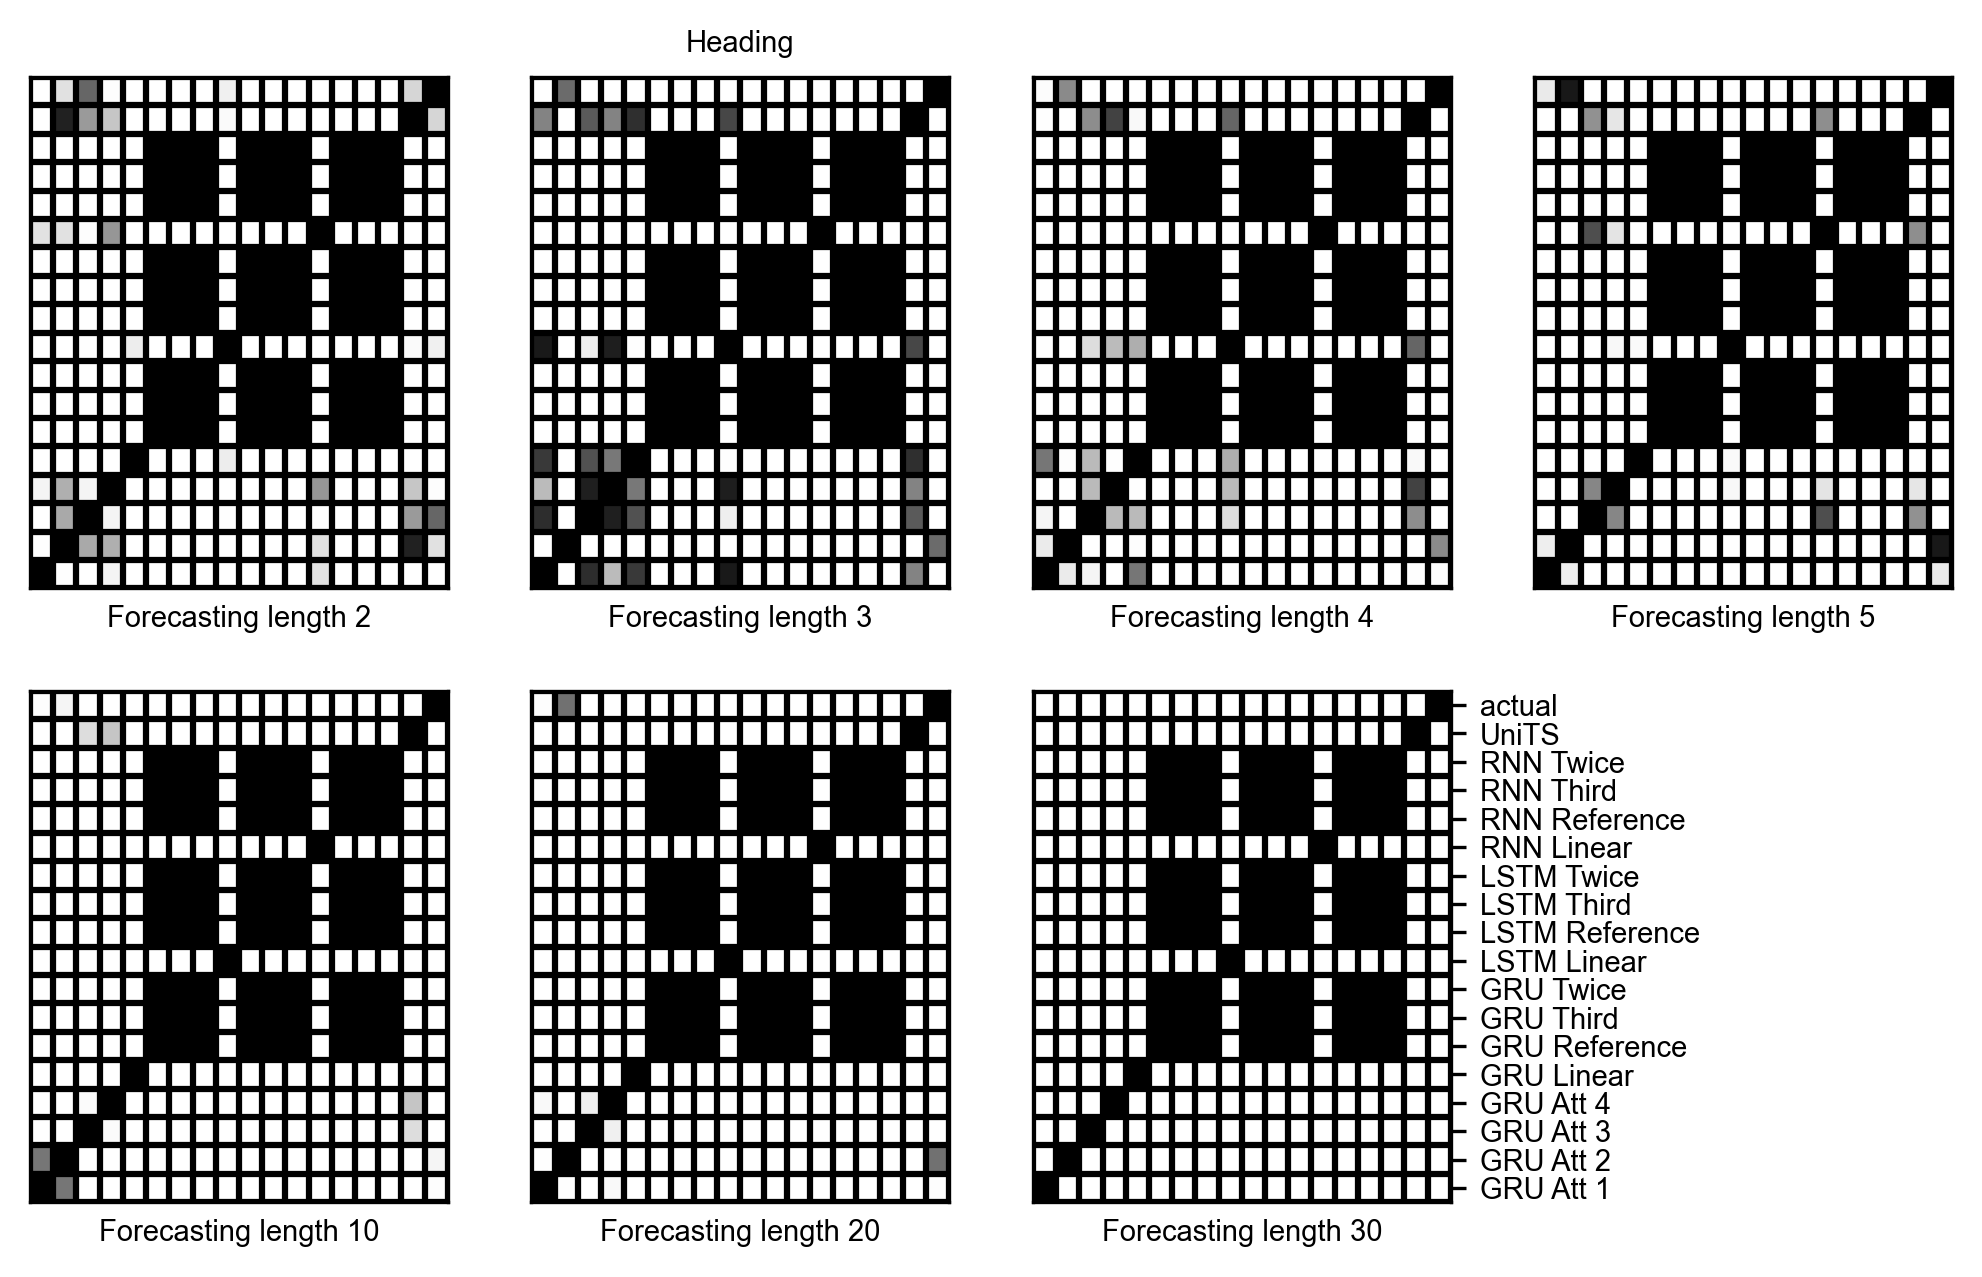
\includegraphics[width = 0.99 \linewidth]{var_direction.png.pdf}
	\caption{The $p$-values for the Mann-Whitney $U$-test on actual and predicted values across k-fold validation datasets for the heading in the k-fold testing datasets using different RNN models, and forecasting times.Darker colors in grayscale represent a higher $p$-value in a range from $0$ to $1$. The values on the secondary diagonal are all equal to $1$ and black beacuse each model is equal to itself.}
	\label{fig:var_direction.png}
\end{figure}

Figure~\ref{fig:best_R2_val} contains the average $R^{2}$ (\%) across k-fold testing datasets using different validation datasets for all variables estimated in nested k-fold cross-validation by different RNN models, and forecasting times.

\begin{figure}[!ht]
	\centering
	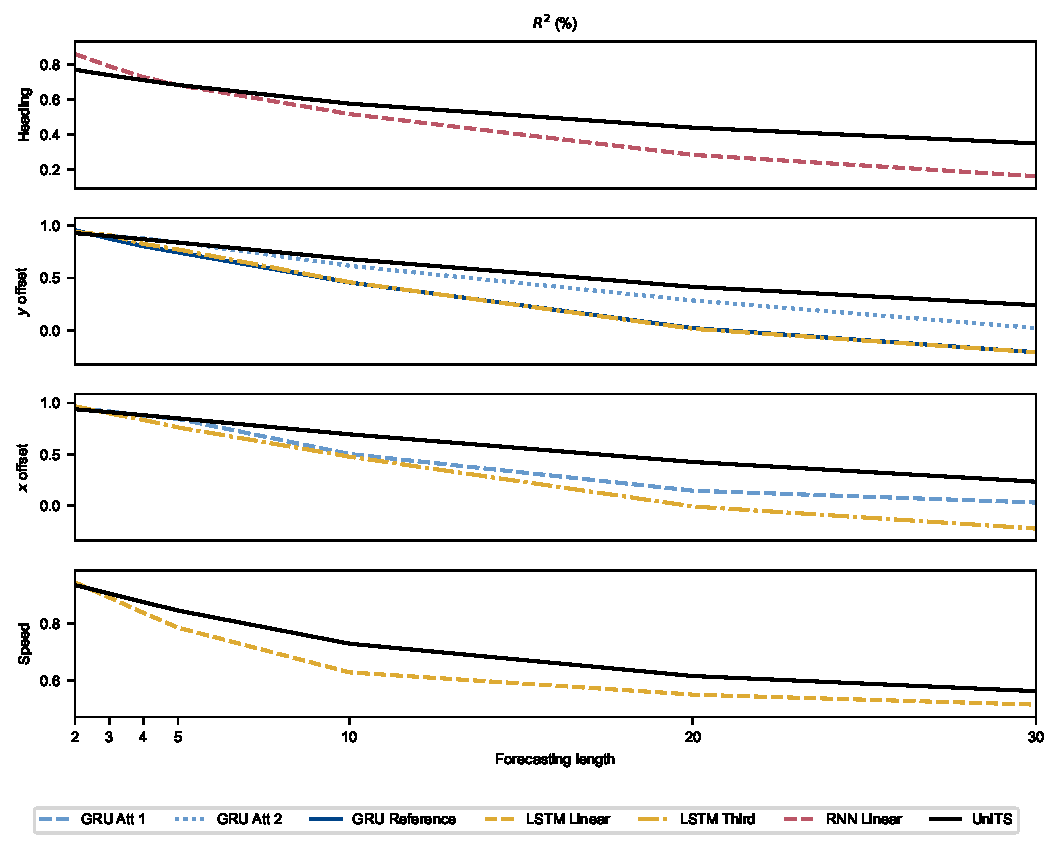
\includegraphics[width = 0.99 \linewidth]{best_R2_val.pdf}
	\caption{The average $R^{2}$ (\%) across k-fold testing datasets using different validation datasets for all variables estimated in nested k-fold cross-validation by different RNN models, and forecasting times.}
	\label{fig:best_R2_val}
\end{figure}

The average $R^{2}$ (\%), with standard deviation in brackets, across k-fold validation datasets for the heading estimated on the k-fold testing datasets by different RNN models, and forecasting times is listed in Table~\ref{tab:best_direction_R2}.

\begin{table}[!ht]
	\centering
	\resizebox{\linewidth}{!}{
		\begin{tabular}{|c|c|c|c|c|c|c|c|}
			\hline
			Model & $2$ $s$ & $3$ $s$ & $4$ $s$ & $5$ $s$ & $10$ $s$ & $20$ $s$ & $30$ $s$ \\ \hline
			\multirow{2}{*}{RNN Linear} & $\mathbf{86.11\%}$ & $\mathbf{79.12\%}$ & $\mathbf{72.83\%}$ & $68.34\%$ & $51.75\%$ & $28.44\%$ & $16.2\%$ \\
			 & \textbf{(}$\mathbf{1.3\%}$\textbf{)} & \textbf{(}$\mathbf{2.11\%}$\textbf{)} & \textbf{(}$\mathbf{2.27\%}$\textbf{)} & ($2.23\%$) & ($3.08\%$) & ($3.04\%$) & ($4.48\%$) \\ \hline
			\multirow{2}{*}{UniTS} & $77.09\%$ & $74.0\%$ & $71.12\%$ & $\mathbf{68.39\%}$ & $\mathbf{57.72\%}$ & $\mathbf{44.0\%}$ & $\mathbf{34.98\%}$ \\
			 & ($1.99\%$) & ($2.25\%$) & ($2.42\%$) & \textbf{(}$\mathbf{2.55\%}$\textbf{)} & \textbf{(}$\mathbf{2.76\%}$\textbf{)} & \textbf{(}$\mathbf{3.21\%}$\textbf{)} & \textbf{(}$\mathbf{3.79\%}$\textbf{)} \\ \hline
		\end{tabular}
	}
	\caption{The average $R^{2}$ (\%), with standard deviation in brackets, across k-fold validation datasets for the heading estimated on the k-fold testing datasets by different RNN models, and forecasting times.}
	\label{tab:best_direction_R2}
\end{table}

The RNN Linear model achieved the highest $R^{2}$ (\%) for heading, and a forecasting time of $2$, $3$, and $4$ $s$ with average values and standard deviation (in brackets) that equal $86.11$\% ($1.3$\%), $79.12$\% ($2.11$\%), and $72.83$\% ($2.27$\%) respectively.

The RNN Linear model does not make statistically significantly different predictions than the GRU Att 1, GRU Att 2, GRU Att 3, GRU Att 4, UniTS, and actual value models for heading using a forecasting time of $2$ $s$, with $p$-values equaling $0.115$, $0.119$, $0.007$, $0.412$, $0.002$, and $0.0$.

The UniTS model achieved the highest $R^{2}$ (\%) for heading, and a forecasting time of $5$, $10$, $20$, and $30$ $s$ with average values and standard deviation (in brackets) that equal $68.39$\% ($2.55$\%), $57.72$\% ($2.76$\%), $44.0$\% ($3.21$\%), and $34.98$\% ($3.79$\%) respectively.

The UniTS model does not make statistically significantly different predictions than the GRU Att 1, GRU Att 3, GRU Att 4, and RNN Linear models for heading using a forecasting time of $5$ $s$, with $p$-values equaling $0.001$, $0.433$, $0.099$, and $0.443$.

The UniTS model does not make statistically significantly different predictions than the GRU Att 3, and GRU Att 4 models for heading using a forecasting time of $10$ $s$, with $p$-values equaling $0.132$, and $0.228$.

Figure~\ref{fig:best_MAE_val} contains the average MAE across k-fold testing datasets using different validation datasets for all variables estimated in nested k-fold cross-validation by different RNN models, and forecasting times.

\begin{figure}[!ht]
	\centering
	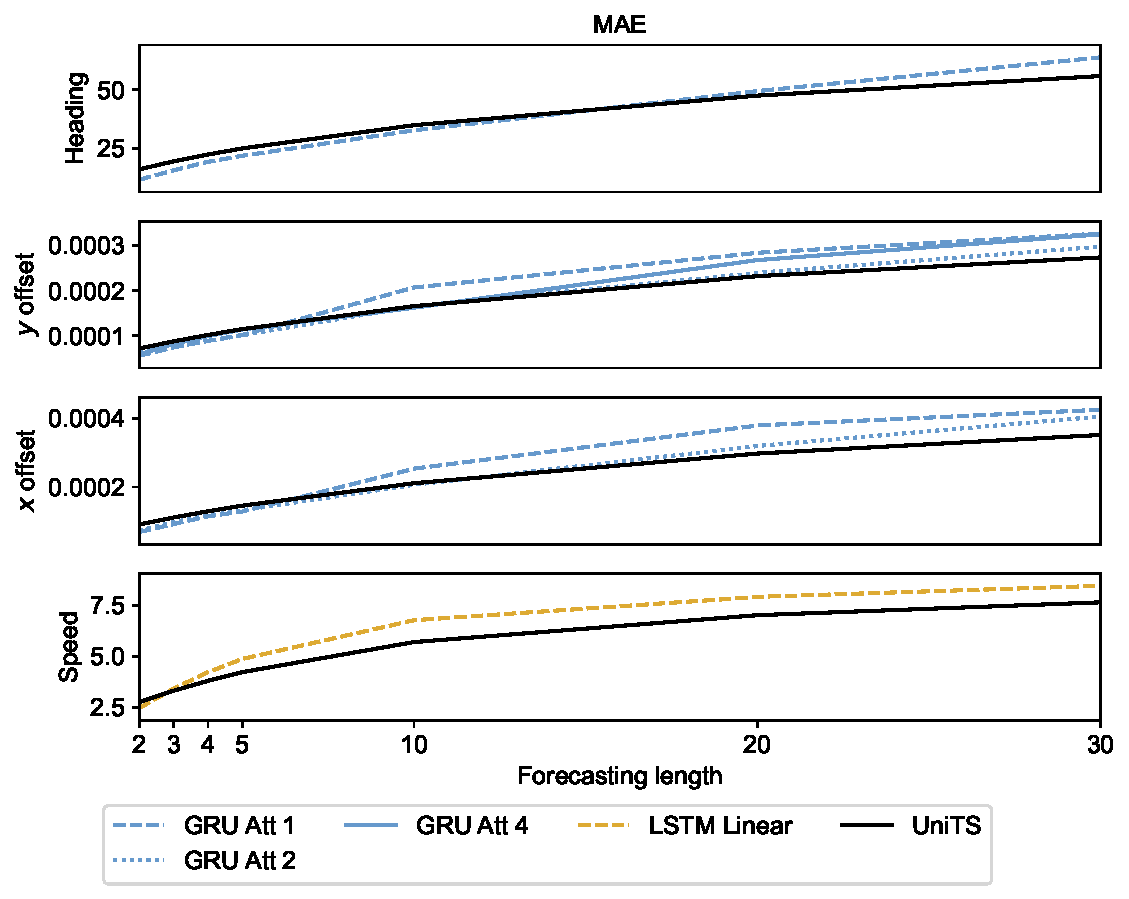
\includegraphics[width = 0.99 \linewidth]{best_MAE_val.pdf}
	\caption{The average MAE across k-fold testing datasets using different validation datasets for all variables estimated in nested k-fold cross-validation by different RNN models, and forecasting times.}
	\label{fig:best_MAE_val}
\end{figure}

The average MAE in $\degree$, with standard deviation in brackets, across k-fold validation datasets for the heading estimated on the k-fold testing datasets by different RNN models, and forecasting times is listed in Table~\ref{tab:best_direction_MAE}.

\begin{table}[!ht]
	\centering
	\resizebox{\linewidth}{!}{
		\begin{tabular}{|c|c|c|c|c|c|c|c|}
			\hline
			Model & $2$ $s$ & $3$ $s$ & $4$ $s$ & $5$ $s$ & $10$ $s$ & $20$ $s$ & $30$ $s$ \\ \hline
			\multirow{2}{*}{GRU Att 1} & $\mathbf{11.77}$ & $\mathbf{15.7}$ & $\mathbf{19.33}$ & $\mathbf{21.9}$ & $\mathbf{32.74}$ & $49.41$ & $63.77$ \\
			 & \textbf{(}$\mathbf{1.29}$\textbf{)} & \textbf{(}$\mathbf{1.63}$\textbf{)} & \textbf{(}$\mathbf{1.67}$\textbf{)} & \textbf{(}$\mathbf{1.75}$\textbf{)} & \textbf{(}$\mathbf{2.14}$\textbf{)} & ($2.48$) & ($10.68$) \\ \hline
			\multirow{2}{*}{UniTS} & $16.17$ & $19.54$ & $22.46$ & $25.04$ & $34.91$ & $\mathbf{47.49}$ & $\mathbf{55.81}$ \\
			 & ($1.21$) & ($1.41$) & ($1.56$) & ($1.68$) & ($2.0$) & \textbf{(}$\mathbf{2.55}$\textbf{)} & \textbf{(}$\mathbf{3.01}$\textbf{)} \\ \hline
		\end{tabular}
	}
	\caption{The average MAE in $\degree$, with standard deviation in brackets, across k-fold validation datasets for the heading estimated on the k-fold testing datasets by different RNN models, and forecasting times.}
	\label{tab:best_direction_MAE}
\end{table}

The GRU Att 1 model achieved the lowest MAE for heading, and a forecasting time of $10$, $2$, $3$, $4$, and $5$ $s$ with average values and standard deviation (in brackets) that equal $32.74$ $\degree$ ($2.14$ $\degree$), $11.77$ $\degree$ ($1.29$ $\degree$), $15.7$ $\degree$ ($1.63$ $\degree$), $19.33$ $\degree$ ($1.67$ $\degree$), and $21.9$ $\degree$ ($1.75$ $\degree$) respectively.

The GRU Att 1 model does not make statistically significantly different predictions than the GRU Att 2, and actual value models for heading using a forecasting time of $10$ $s$, with $p$-values equaling $0.535$, and $0.008$.

The GRU Att 1 model does not make statistically significantly different predictions than the GRU Att 2, GRU Att 4, RNN Linear, and UniTS models for heading using a forecasting time of $2$ $s$, with $p$-values equaling $0.002$, $0.042$, $0.115$, and $0.001$.

The GRU Att 1 model does not make statistically significantly different predictions than the GRU Att 3, GRU Att 4, GRU Linear, LSTM Linear, and UniTS models for heading using a forecasting time of $3$ $s$, with $p$-values equaling $0.823$, $0.958$, $0.776$, $0.904$, and $0.485$.

The GRU Att 1 model does not make statistically significantly different predictions than the GRU Att 2, GRU Att 3, GRU Att 4, GRU Linear, LSTM Linear, UniTS, and actual value models for heading using a forecasting time of $4$ $s$, with $p$-values equaling $0.078$, $0.041$, $0.002$, $0.538$, $0.002$, $0.005$, and $0.011$.

The GRU Att 1 model does not make statistically significantly different predictions than the GRU Att 2, UniTS, and actual value models for heading using a forecasting time of $5$ $s$, with $p$-values equaling $0.068$, $0.001$, and $0.081$.

The UniTS model achieved the lowest MAE for heading, and a forecasting time of $20$, and $30$ $s$ with average values and standard deviation (in brackets) that equal $47.49$ $\degree$ ($2.55$ $\degree$), and $55.81$ $\degree$ ($3.01$ $\degree$) respectively.

\subsection{Results for $y$ Offset}
%\label{subsec:latitude_no_abs_results}
%\vspace{10pt}

Figure~\ref{fig:var_latitude_no_abs.png} represents the $p$-values for the Mann-Whitney $U$-test on actual and predicted values across k-fold validation datasets for the $y$ offset in the k-fold testing datasets using different RNN models, and forecasting times.Darker colors in grayscale represent a higher $p$-value in a range from $0$ to $1$. The values on the secondary diagonal are all equal to $1$ and black beacuse each model is equal to itself.

\begin{figure}[!ht]
	\centering
	\includegraphics[width = 0.99 \linewidth]{var_latitude_no_abs.png.pdf}
	\caption{The $p$-values for the Mann-Whitney $U$-test on actual and predicted values across k-fold validation datasets for the $y$ offset in the k-fold testing datasets using different RNN models, and forecasting times.Darker colors in grayscale represent a higher $p$-value in a range from $0$ to $1$. The values on the secondary diagonal are all equal to $1$ and black beacuse each model is equal to itself.}
	\label{fig:var_latitude_no_abs.png}
\end{figure}

The average $R^{2}$ (\%), with standard deviation in brackets, across k-fold validation datasets for the $y$ offset estimated on the k-fold testing datasets by different RNN models, and forecasting times is listed in Table~\ref{tab:best_latitude_no_abs_R2}.

\begin{table}[!ht]
	\centering
	\resizebox{\linewidth}{!}{
		\begin{tabular}{|c|c|c|c|c|c|c|c|}
			\hline
			Model & $2$ $s$ & $3$ $s$ & $4$ $s$ & $5$ $s$ & $10$ $s$ & $20$ $s$ & $30$ $s$ \\ \hline
			\multirow{2}{*}{GRU Att 2} & $93.23\%$ & $90.0\%$ & $\mathbf{87.69\%}$ & $\mathbf{84.05\%}$ & $61.6\%$ & $28.71\%$ & $2.39\%$ \\
			 & ($1.51\%$) & ($2.05\%$) & \textbf{(}$\mathbf{1.72\%}$\textbf{)} & \textbf{(}$\mathbf{1.93\%}$\textbf{)} & ($3.4\%$) & ($6.2\%$) & ($8.4\%$) \\ \hline
			\multirow{2}{*}{GRU Reference} & $\mathbf{95.61\%}$ & $87.54\%$ & $80.31\%$ & $74.42\%$ & $45.82\%$ & $2.42\%$ & $-20.58\%$ \\
			 & \textbf{(}$\mathbf{2.14\%}$\textbf{)} & ($4.07\%$) & ($4.96\%$) & ($4.09\%$) & ($4.34\%$) & ($5.99\%$) & ($7.07\%$) \\ \hline
			\multirow{2}{*}{LSTM Third} & $93.81\%$ & $\mathbf{90.91\%}$ & $82.5\%$ & $77.25\%$ & $46.06\%$ & $1.72\%$ & $-20.76\%$ \\
			 & ($3.93\%$) & \textbf{(}$\mathbf{5.23\%}$\textbf{)} & ($8.75\%$) & ($5.43\%$) & ($3.94\%$) & ($5.94\%$) & ($9.82\%$) \\ \hline
			\multirow{2}{*}{UniTS} & $92.75\%$ & $89.96\%$ & $86.92\%$ & $83.77\%$ & $\mathbf{68.0\%}$ & $\mathbf{41.68\%}$ & $\mathbf{24.17\%}$ \\
			 & ($1.98\%$) & ($1.67\%$) & ($1.63\%$) & ($1.67\%$) & \textbf{(}$\mathbf{2.31\%}$\textbf{)} & \textbf{(}$\mathbf{3.95\%}$\textbf{)} & \textbf{(}$\mathbf{4.68\%}$\textbf{)} \\ \hline
		\end{tabular}
	}
	\caption{The average $R^{2}$ (\%), with standard deviation in brackets, across k-fold validation datasets for the $y$ offset estimated on the k-fold testing datasets by different RNN models, and forecasting times.}
	\label{tab:best_latitude_no_abs_R2}
\end{table}

The GRU Att 2 model achieved the highest $R^{2}$ (\%) for $y$ offset, and a forecasting time of $4$, and $5$ $s$ with average values and standard deviation (in brackets) that equal $87.69$\% ($1.72$\%), and $84.05$\% ($1.93$\%) respectively.

The GRU Att 2 model does not make statistically significantly different predictions than the GRU Att 1, GRU Att 3, GRU Att 4, GRU Third, UniTS, and actual value models for $y$ offset using a forecasting time of $4$ $s$, with $p$-values equaling $0.178$, $0.219$, $0.236$, $0.001$, $0.0$, and $0.509$.

The GRU Att 2 model does not make statistically significantly different predictions than the GRU Att 1, GRU Att 3, GRU Att 4, UniTS, and actual value models for $y$ offset using a forecasting time of $5$ $s$, with $p$-values equaling $0.069$, $0.153$, $0.789$, $0.018$, and $0.209$.

The GRU Reference model achieved the highest $R^{2}$ (\%) for $y$ offset, and a forecasting time of $2$ $s$ with an average value and standard deviation (in brackets) that equals $95.61$\% ($2.14$\%).

The LSTM Third model achieved the highest $R^{2}$ (\%) for $y$ offset, and a forecasting time of $3$ $s$ with an average value and standard deviation (in brackets) that equals $90.91$\% ($5.23$\%).

The UniTS model achieved the highest $R^{2}$ (\%) for $y$ offset, and a forecasting time of $10$, $20$, and $30$ $s$ with average values and standard deviation (in brackets) that equal $68.0$\% ($2.31$\%), $41.68$\% ($3.95$\%), and $24.17$\% ($4.68$\%) respectively.

The UniTS model does not make statistically significantly different predictions than the GRU Att 2, GRU Att 3, LSTM Third, and actual value models for $y$ offset using a forecasting time of $10$ $s$, with $p$-values equaling $0.664$, $0.052$, $0.068$, and $0.019$.

The UniTS model does not make statistically significantly different predictions than the GRU Att 4, GRU Third, RNN Twice, and actual value models for $y$ offset using a forecasting time of $20$ $s$, with $p$-values equaling $0.054$, $0.002$, $0.464$, and $0.538$.

The UniTS model does not make statistically significantly different predictions than the GRU Att 2, GRU Att 4, and actual value models for $y$ offset using a forecasting time of $30$ $s$, with $p$-values equaling $0.093$, $0.472$, and $0.152$.

The average MAE in $\degree$ ($\times 10^{-5}$), with standard deviation in brackets, across k-fold validation datasets for the $y$ offset estimated on the k-fold testing datasets by different RNN models, and forecasting times is listed in Table~\ref{tab:best_latitude_no_abs_MAE}.

\begin{table}[!ht]
	\centering
	\resizebox{\linewidth}{!}{
		\begin{tabular}{|c|c|c|c|c|c|c|c|}
			\hline
			Model & $2$ $s$ & $3$ $s$ & $4$ $s$ & $5$ $s$ & $10$ $s$ & $20$ $s$ & $30$ $s$ \\ \hline
			\multirow{2}{*}{GRU Att 1} & $\mathbf{5.558}$ & $\mathbf{7.454}$ & $8.885$ & $10.171$ & $20.701$ & $28.391$ & $32.677$ \\
			 & \textbf{(}$\mathbf{0.492}$\textbf{)} & \textbf{(}$\mathbf{0.708}$\textbf{)} & ($0.707$) & ($0.941$) & ($4.684$) & ($3.632$) & ($2.745$) \\ \hline
			\multirow{2}{*}{GRU Att 2} & $6.187$ & $7.917$ & $\mathbf{8.816}$ & $\mathbf{10.118}$ & $16.546$ & $23.948$ & $29.776$ \\
			 & ($0.608$) & ($1.082$) & \textbf{(}$\mathbf{0.762}$\textbf{)} & \textbf{(}$\mathbf{0.997}$\textbf{)} & ($1.513$) & ($2.1$) & ($2.891$) \\ \hline
			\multirow{2}{*}{GRU Att 4} & $5.863$ & $8.231$ & $9.942$ & $11.388$ & $\mathbf{16.223}$ & $26.774$ & $32.495$ \\
			 & ($0.526$) & ($0.708$) & ($0.854$) & ($1.044$) & \textbf{(}$\mathbf{1.953}$\textbf{)} & ($4.307$) & ($3.099$) \\ \hline
			\multirow{2}{*}{UniTS} & $7.176$ & $8.763$ & $10.181$ & $11.466$ & $16.562$ & $\mathbf{23.209}$ & $\mathbf{27.355}$ \\
			 & ($0.607$) & ($0.759$) & ($0.88$) & ($0.988$) & ($1.426$) & \textbf{(}$\mathbf{2.001}$\textbf{)} & \textbf{(}$\mathbf{2.3}$\textbf{)} \\ \hline
		\end{tabular}
	}
	\caption{The average MAE in $\degree$ ($\times 10^{-5}$), with standard deviation in brackets, across k-fold validation datasets for the $y$ offset estimated on the k-fold testing datasets by different RNN models, and forecasting times.}
	\label{tab:best_latitude_no_abs_MAE}
\end{table}

The GRU Att 1 model achieved the lowest MAE for $y$ offset, and a forecasting time of $2$, and $3$ $s$ with average values and standard deviation (in brackets) that equal $5.558 \times 10^{-5}$ $\degree$ ($0.492 \times 10^{-5}$ $\degree$), and $7.454 \times 10^{-5}$ $\degree$ ($0.708 \times 10^{-5}$ $\degree$) respectively.

The GRU Att 1 model does not make statistically significantly different predictions than the GRU Att 2, GRU Att 3, GRU Att 4, UniTS, and actual value models for $y$ offset using a forecasting time of $2$ $s$, with $p$-values equaling $0.948$, $0.048$, $0.378$, $0.011$, and $0.494$.

The GRU Att 1 model does not make statistically significantly different predictions than the GRU Att 2, GRU Att 3, GRU Att 4, LSTM Linear, LSTM Twice, and actual value models for $y$ offset using a forecasting time of $3$ $s$, with $p$-values equaling $0.766$, $0.273$, $0.7$, $0.017$, $0.102$, and $0.453$.

The GRU Att 2 model achieved the lowest MAE for $y$ offset, and a forecasting time of $4$, and $5$ $s$ with average values and standard deviation (in brackets) that equal $8.816 \times 10^{-5}$ $\degree$ ($0.762 \times 10^{-5}$ $\degree$), and $10.118 \times 10^{-5}$ $\degree$ ($0.997 \times 10^{-5}$ $\degree$) respectively.

The GRU Att 2 model does not make statistically significantly different predictions than the GRU Att 1, GRU Att 3, GRU Att 4, GRU Third, UniTS, and actual value models for $y$ offset using a forecasting time of $4$ $s$, with $p$-values equaling $0.178$, $0.219$, $0.236$, $0.001$, $0.0$, and $0.509$.

The GRU Att 2 model does not make statistically significantly different predictions than the GRU Att 1, GRU Att 3, GRU Att 4, UniTS, and actual value models for $y$ offset using a forecasting time of $5$ $s$, with $p$-values equaling $0.069$, $0.153$, $0.789$, $0.018$, and $0.209$.

The GRU Att 4 model achieved the lowest MAE for $y$ offset, and a forecasting time of $10$ $s$ with an average value and standard deviation (in brackets) that equals $16.223 \times 10^{-5}$ $\degree$ ($1.953 \times 10^{-5}$ $\degree$).

The GRU Att 4 model does not make statistically significantly different predictions than the GRU Att 2, LSTM Linear, LSTM Third, and actual value models for $y$ offset using a forecasting time of $10$ $s$, with $p$-values equaling $0.001$, $0.0$, $0.006$, and $0.214$.

The UniTS model achieved the lowest MAE for $y$ offset, and a forecasting time of $20$, and $30$ $s$ with average values and standard deviation (in brackets) that equal $23.209 \times 10^{-5}$ $\degree$ ($2.001 \times 10^{-5}$ $\degree$), and $27.355 \times 10^{-5}$ $\degree$ ($2.3 \times 10^{-5}$ $\degree$) respectively.

The UniTS model does not make statistically significantly different predictions than the GRU Att 4, GRU Third, RNN Twice, and actual value models for $y$ offset using a forecasting time of $20$ $s$, with $p$-values equaling $0.054$, $0.002$, $0.464$, and $0.538$.

The UniTS model does not make statistically significantly different predictions than the GRU Att 2, GRU Att 4, and actual value models for $y$ offset using a forecasting time of $30$ $s$, with $p$-values equaling $0.093$, $0.472$, and $0.152$.

\subsection{Results for $x$ Offset}
%\label{subsec:longitude_no_abs_results}
%\vspace{10pt}

Figure~\ref{fig:var_longitude_no_abs.png} represents the $p$-values for the Mann-Whitney $U$-test on actual and predicted values across k-fold validation datasets for the $x$ offset in the k-fold testing datasets using different RNN models, and forecasting times.Darker colors in grayscale represent a higher $p$-value in a range from $0$ to $1$. The values on the secondary diagonal are all equal to $1$ and black beacuse each model is equal to itself.

\begin{figure}[!ht]
	\centering
	\includegraphics[width = 0.99 \linewidth]{var_longitude_no_abs.png.pdf}
	\caption{The $p$-values for the Mann-Whitney $U$-test on actual and predicted values across k-fold validation datasets for the $x$ offset in the k-fold testing datasets using different RNN models, and forecasting times.Darker colors in grayscale represent a higher $p$-value in a range from $0$ to $1$. The values on the secondary diagonal are all equal to $1$ and black beacuse each model is equal to itself.}
	\label{fig:var_longitude_no_abs.png}
\end{figure}

The average $R^{2}$ (\%), with standard deviation in brackets, across k-fold validation datasets for the $x$ offset estimated on the k-fold testing datasets by different RNN models, and forecasting times is listed in Table~\ref{tab:best_longitude_no_abs_R2}.

\begin{table}[!ht]
	\centering
	\resizebox{\linewidth}{!}{
		\begin{tabular}{|c|c|c|c|c|c|c|c|}
			\hline
			Model & $2$ $s$ & $3$ $s$ & $4$ $s$ & $5$ $s$ & $10$ $s$ & $20$ $s$ & $30$ $s$ \\ \hline
			\multirow{2}{*}{GRU Att 1} & $95.29\%$ & $\mathbf{91.83\%}$ & $87.74\%$ & $84.62\%$ & $50.34\%$ & $14.63\%$ & $3.01\%$ \\
			 & ($0.92\%$) & \textbf{(}$\mathbf{1.53\%}$\textbf{)} & ($2.02\%$) & ($2.12\%$) & ($14.06\%$) & ($5.96\%$) & ($13.0\%$) \\ \hline
			\multirow{2}{*}{LSTM Third} & $\mathbf{96.88\%}$ & $89.96\%$ & $83.59\%$ & $76.3\%$ & $47.76\%$ & $-0.74\%$ & $-22.31\%$ \\
			 & \textbf{(}$\mathbf{1.13\%}$\textbf{)} & ($3.73\%$) & ($4.38\%$) & ($4.29\%$) & ($4.45\%$) & ($5.66\%$) & ($4.66\%$) \\ \hline
			\multirow{2}{*}{UniTS} & $93.99\%$ & $91.18\%$ & $\mathbf{88.19\%}$ & $\mathbf{85.09\%}$ & $\mathbf{69.54\%}$ & $\mathbf{42.6\%}$ & $\mathbf{23.39\%}$ \\
			 & ($0.83\%$) & ($1.05\%$) & \textbf{(}$\mathbf{1.32\%}$\textbf{)} & \textbf{(}$\mathbf{1.57\%}$\textbf{)} & \textbf{(}$\mathbf{2.54\%}$\textbf{)} & \textbf{(}$\mathbf{3.68\%}$\textbf{)} & \textbf{(}$\mathbf{4.0\%}$\textbf{)} \\ \hline
		\end{tabular}
	}
	\caption{The average $R^{2}$ (\%), with standard deviation in brackets, across k-fold validation datasets for the $x$ offset estimated on the k-fold testing datasets by different RNN models, and forecasting times.}
	\label{tab:best_longitude_no_abs_R2}
\end{table}

The GRU Att 1 model achieved the highest $R^{2}$ (\%) for $x$ offset, and a forecasting time of $3$ $s$ with an average value and standard deviation (in brackets) that equals $91.83$\% ($1.53$\%).

The GRU Att 1 model does not make statistically significantly different predictions than the GRU Att 2, GRU Att 3, GRU Att 4, GRU Linear, LSTM Linear, RNN Third, and actual value models for $x$ offset using a forecasting time of $3$ $s$, with $p$-values equaling $0.175$, $0.968$, $0.571$, $0.304$, $0.004$, $0.023$, and $0.9$.

The LSTM Third model achieved the highest $R^{2}$ (\%) for $x$ offset, and a forecasting time of $2$ $s$ with an average value and standard deviation (in brackets) that equals $96.88$\% ($1.13$\%).

The LSTM Third model does not make statistically significantly different predictions than the LSTM Reference model for $x$ offset using a forecasting time of $2$ $s$, with a $p$-value equaling $0.063$.

The UniTS model achieved the highest $R^{2}$ (\%) for $x$ offset, and a forecasting time of $4$, $5$, $10$, $20$, and $30$ $s$ with average values and standard deviation (in brackets) that equal $88.19$\% ($1.32$\%), $85.09$\% ($1.57$\%), $69.54$\% ($2.54$\%), $42.6$\% ($3.68$\%), and $23.39$\% ($4.0$\%) respectively.

The UniTS model does not make statistically significantly different predictions than the GRU Att 3, and actual value models for $x$ offset using a forecasting time of $4$ $s$, with $p$-values equaling $0.002$, and $0.003$.

The UniTS model does not make statistically significantly different predictions than the GRU Att 3, GRU Twice, LSTM Third, and actual value models for $x$ offset using a forecasting time of $5$ $s$, with $p$-values equaling $0.016$, $0.003$, $0.063$, and $0.005$.

The UniTS model does not make statistically significantly different predictions than the GRU Att 2, GRU Att 3, LSTM Reference, LSTM Twice, and actual value models for $x$ offset using a forecasting time of $10$ $s$, with $p$-values equaling $0.046$, $0.54$, $0.007$, $0.001$, and $0.0$.

The UniTS model does not make statistically significantly different predictions than the GRU Att 3, and GRU Third models for $x$ offset using a forecasting time of $20$ $s$, with $p$-values equaling $0.976$, and $0.204$.

The average MAE in $\degree$ ($\times 10^{-5}$), with standard deviation in brackets, across k-fold validation datasets for the $x$ offset estimated on the k-fold testing datasets by different RNN models, and forecasting times is listed in Table~\ref{tab:best_longitude_no_abs_MAE}.

\begin{table}[!ht]
	\centering
	\resizebox{\linewidth}{!}{
		\begin{tabular}{|c|c|c|c|c|c|c|c|}
			\hline
			Model & $2$ $s$ & $3$ $s$ & $4$ $s$ & $5$ $s$ & $10$ $s$ & $20$ $s$ & $30$ $s$ \\ \hline
			\multirow{2}{*}{GRU Att 1} & $\mathbf{6.81}$ & $\mathbf{9.13}$ & $\mathbf{11.39}$ & $\mathbf{12.77}$ & $25.31$ & $37.95$ & $42.58$ \\
			 & \textbf{(}$\mathbf{0.85}$\textbf{)} & \textbf{(}$\mathbf{1.09}$\textbf{)} & \textbf{(}$\mathbf{1.48}$\textbf{)} & \textbf{(}$\mathbf{1.41}$\textbf{)} & ($5.26$) & ($3.28$) & ($3.71$) \\ \hline
			\multirow{2}{*}{GRU Att 2} & $7.15$ & $9.67$ & $11.58$ & $13.14$ & $\mathbf{20.61}$ & $31.95$ & $40.63$ \\
			 & ($0.86$) & ($1.3$) & ($1.44$) & ($2.01$) & \textbf{(}$\mathbf{2.81}$\textbf{)} & ($3.97$) & ($4.81$) \\ \hline
			\multirow{2}{*}{UniTS} & $9.01$ & $11.04$ & $12.85$ & $14.49$ & $21.05$ & $\mathbf{29.73}$ & $\mathbf{35.17}$ \\
			 & ($0.96$) & ($1.19$) & ($1.38$) & ($1.55$) & ($2.2$) & \textbf{(}$\mathbf{3.04}$\textbf{)} & \textbf{(}$\mathbf{3.37}$\textbf{)} \\ \hline
		\end{tabular}
	}
	\caption{The average MAE in $\degree$ ($\times 10^{-5}$), with standard deviation in brackets, across k-fold validation datasets for the $x$ offset estimated on the k-fold testing datasets by different RNN models, and forecasting times.}
	\label{tab:best_longitude_no_abs_MAE}
\end{table}

The GRU Att 1 model achieved the lowest MAE for $x$ offset, and a forecasting time of $2$, $3$, $4$, and $5$ $s$ with average values and standard deviation (in brackets) that equal $6.81 \times 10^{-5}$ $\degree$ ($0.85 \times 10^{-5}$ $\degree$), $9.13 \times 10^{-5}$ $\degree$ ($1.09 \times 10^{-5}$ $\degree$), $11.39 \times 10^{-5}$ $\degree$ ($1.48 \times 10^{-5}$ $\degree$), and $12.77 \times 10^{-5}$ $\degree$ ($1.41 \times 10^{-5}$ $\degree$) respectively.

The GRU Att 1 model does not make statistically significantly different predictions than the GRU Att 2, GRU Att 3, GRU Att 4, LSTM Linear, LSTM Twice, UniTS, and actual value models for $x$ offset using a forecasting time of $2$ $s$, with $p$-values equaling $0.954$, $0.611$, $0.524$, $0.052$, $0.02$, $0.265$, and $0.412$.

The GRU Att 1 model does not make statistically significantly different predictions than the GRU Att 2, GRU Att 3, GRU Att 4, GRU Linear, LSTM Linear, RNN Third, and actual value models for $x$ offset using a forecasting time of $3$ $s$, with $p$-values equaling $0.175$, $0.968$, $0.571$, $0.304$, $0.004$, $0.023$, and $0.9$.

The GRU Att 1 model does not make statistically significantly different predictions than the GRU Att 2, GRU Att 3, GRU Att 4, LSTM Twice, RNN Linear, and actual value models for $x$ offset using a forecasting time of $4$ $s$, with $p$-values equaling $0.063$, $0.45$, $0.756$, $0.728$, $0.054$, and $0.417$.

The GRU Att 1 model does not make statistically significantly different predictions than the GRU Att 2, GRU Att 3, GRU Att 4, and actual value models for $x$ offset using a forecasting time of $5$ $s$, with $p$-values equaling $0.031$, $0.332$, $0.574$, and $0.595$.

The GRU Att 2 model achieved the lowest MAE for $x$ offset, and a forecasting time of $10$ $s$ with an average value and standard deviation (in brackets) that equals $20.61 \times 10^{-5}$ $\degree$ ($2.81 \times 10^{-5}$ $\degree$).

The GRU Att 2 model does not make statistically significantly different predictions than the GRU Att 3, LSTM Third, UniTS, and actual value models for $x$ offset using a forecasting time of $10$ $s$, with $p$-values equaling $0.055$, $0.145$, $0.046$, and $0.037$.

The UniTS model achieved the lowest MAE for $x$ offset, and a forecasting time of $20$, and $30$ $s$ with average values and standard deviation (in brackets) that equal $29.73 \times 10^{-5}$ $\degree$ ($3.04 \times 10^{-5}$ $\degree$), and $35.17 \times 10^{-5}$ $\degree$ ($3.37 \times 10^{-5}$ $\degree$) respectively.

The UniTS model does not make statistically significantly different predictions than the GRU Att 3, and GRU Third models for $x$ offset using a forecasting time of $20$ $s$, with $p$-values equaling $0.976$, and $0.204$.

\subsection{Results for Speed}
%\label{subsec:speed_results}
%\vspace{10pt}

Figure~\ref{fig:var_speed.png} represents the $p$-values for the Mann-Whitney $U$-test on actual and predicted values across k-fold validation datasets for the speed in the k-fold testing datasets using different RNN models, and forecasting times.Darker colors in grayscale represent a higher $p$-value in a range from $0$ to $1$. The values on the secondary diagonal are all equal to $1$ and black beacuse each model is equal to itself.

\begin{figure}[!ht]
	\centering
	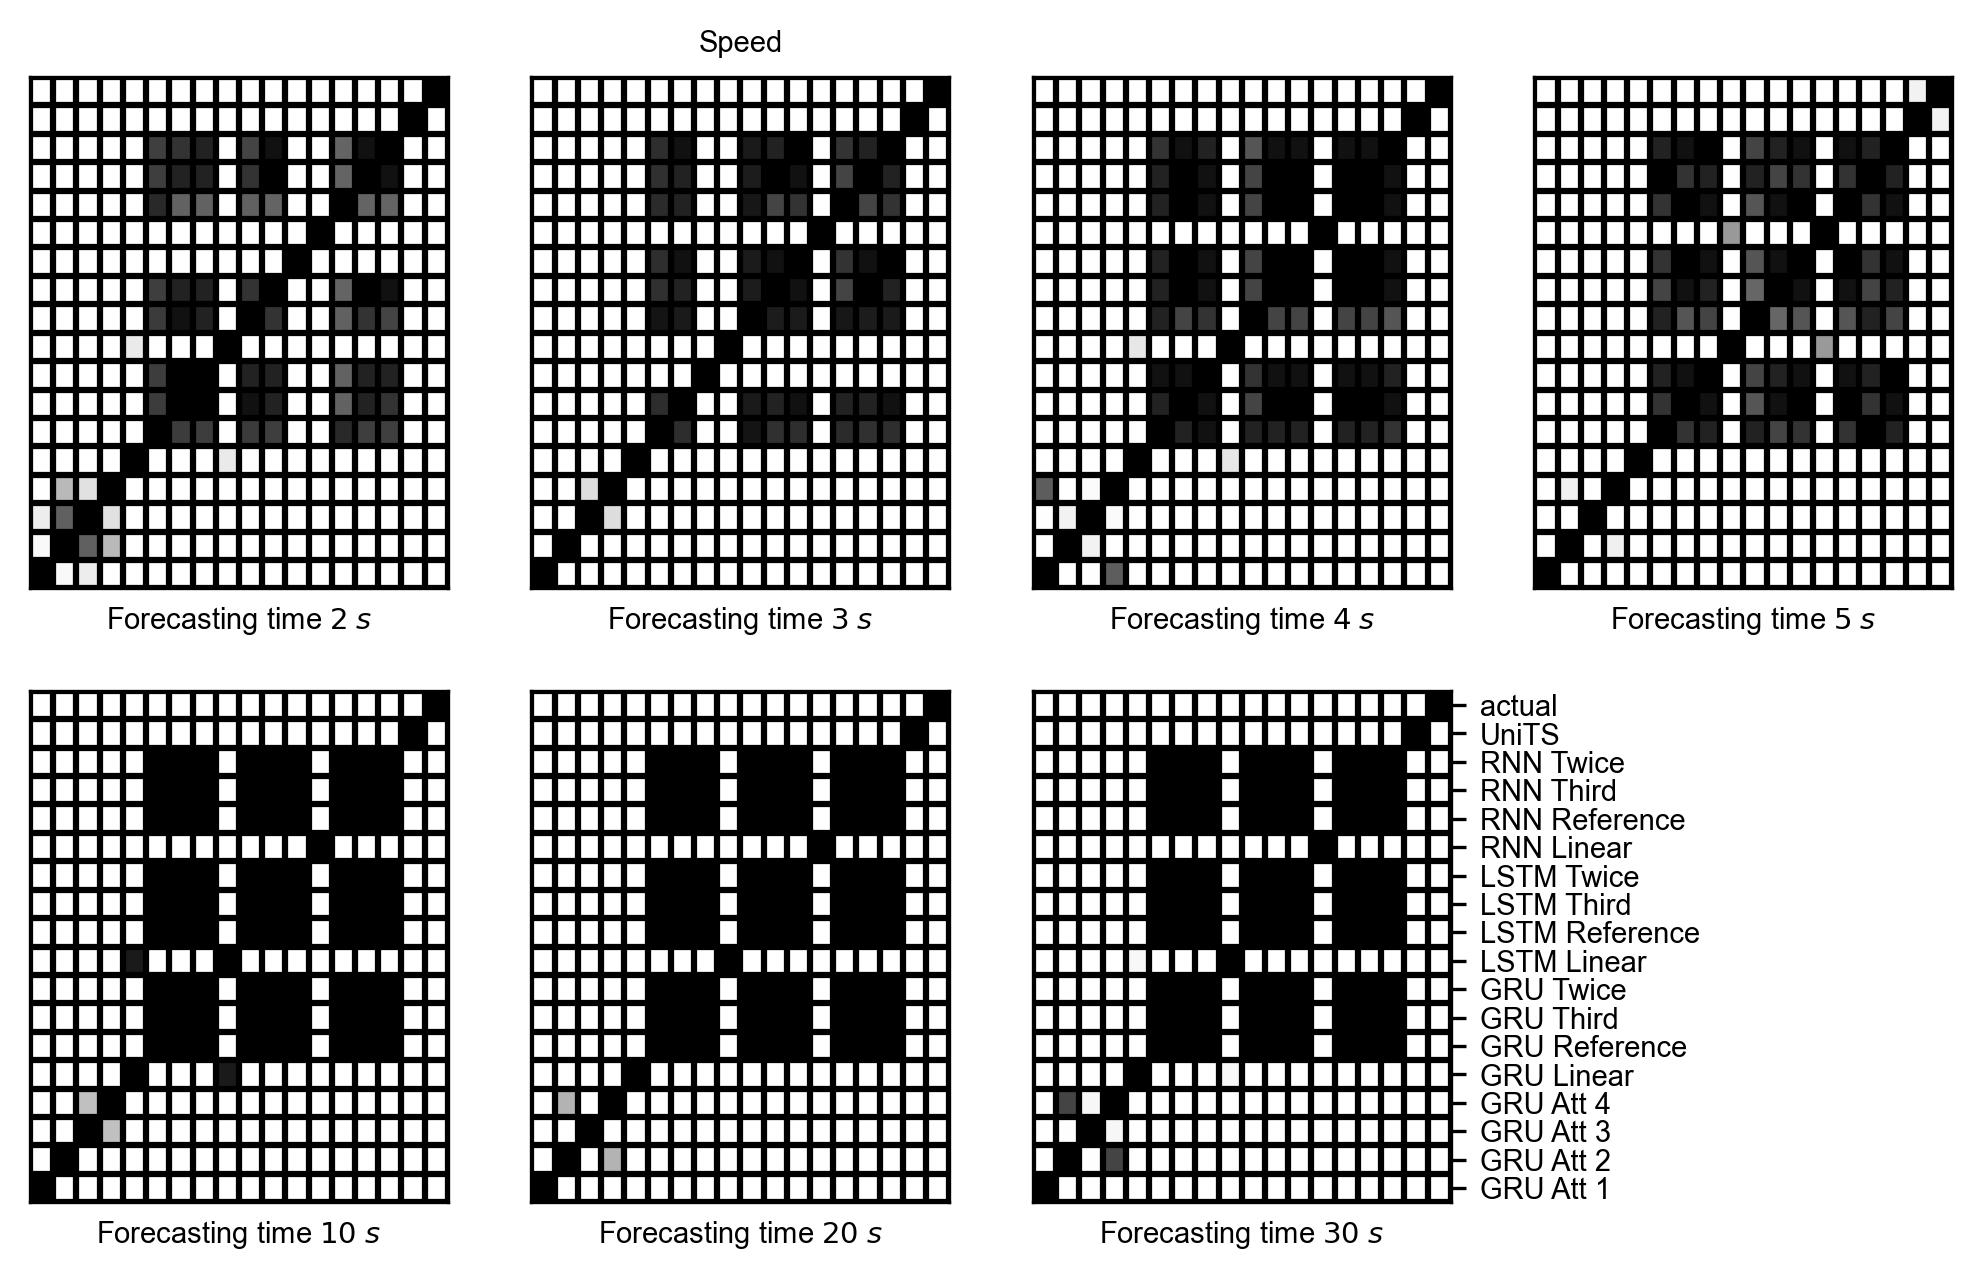
\includegraphics[width = 0.99 \linewidth]{var_speed.png.pdf}
	\caption{The $p$-values for the Mann-Whitney $U$-test on actual and predicted values across k-fold validation datasets for the speed in the k-fold testing datasets using different RNN models, and forecasting times.Darker colors in grayscale represent a higher $p$-value in a range from $0$ to $1$. The values on the secondary diagonal are all equal to $1$ and black beacuse each model is equal to itself.}
	\label{fig:var_speed.png}
\end{figure}

The average $R^{2}$ (\%), with standard deviation in brackets, across k-fold validation datasets for the speed estimated on the k-fold testing datasets by different RNN models, and forecasting times is listed in Table~\ref{tab:best_speed_R2}.

\begin{table}[!ht]
	\centering
	\resizebox{\linewidth}{!}{
		\begin{tabular}{|c|c|c|c|c|c|c|c|}
			\hline
			Model & $2$ $s$ & $3$ $s$ & $4$ $s$ & $5$ $s$ & $10$ $s$ & $20$ $s$ & $30$ $s$ \\ \hline
			\multirow{2}{*}{LSTM Linear} & $\mathbf{94.39\%}$ & $89.11\%$ & $83.69\%$ & $78.54\%$ & $62.8\%$ & $54.98\%$ & $51.44\%$ \\
			 & \textbf{(}$\mathbf{0.63\%}$\textbf{)} & ($1.3\%$) & ($1.83\%$) & ($2.27\%$) & ($3.95\%$) & ($4.2\%$) & ($4.16\%$) \\ \hline
			\multirow{2}{*}{UniTS} & $93.45\%$ & $\mathbf{90.5\%}$ & $\mathbf{87.48\%}$ & $\mathbf{84.54\%}$ & $\mathbf{72.89\%}$ & $\mathbf{61.53\%}$ & $\mathbf{56.21\%}$ \\
			 & ($0.64\%$) & \textbf{(}$\mathbf{0.92\%}$\textbf{)} & \textbf{(}$\mathbf{1.21\%}$\textbf{)} & \textbf{(}$\mathbf{1.49\%}$\textbf{)} & \textbf{(}$\mathbf{2.68\%}$\textbf{)} & \textbf{(}$\mathbf{3.89\%}$\textbf{)} & \textbf{(}$\mathbf{3.92\%}$\textbf{)} \\ \hline
		\end{tabular}
	}
	\caption{The average $R^{2}$ (\%), with standard deviation in brackets, across k-fold validation datasets for the speed estimated on the k-fold testing datasets by different RNN models, and forecasting times.}
	\label{tab:best_speed_R2}
\end{table}

The LSTM Linear model achieved the highest $R^{2}$ (\%) for speed, and a forecasting time of $2$ $s$ with an average value and standard deviation (in brackets) that equals $94.39$\% ($0.63$\%).

The LSTM Linear model does not make statistically significantly different predictions than the GRU Linear model for speed using a forecasting time of $2$ $s$, with a $p$-value equaling $0.084$.

The UniTS model achieved the highest $R^{2}$ (\%) for speed, and a forecasting time of $3$, $4$, $5$, $10$, $20$, and $30$ $s$ with average values and standard deviation (in brackets) that equal $90.5$\% ($0.92$\%), $87.48$\% ($1.21$\%), $84.54$\% ($1.49$\%), $72.89$\% ($2.68$\%), $61.53$\% ($3.89$\%), and $56.21$\% ($3.92$\%) respectively.

The UniTS model does not make statistically significantly different predictions than the actual value model for speed using a forecasting time of $4$ $s$, with a $p$-value equaling $0.002$.

The UniTS model does not make statistically significantly different predictions than the actual value model for speed using a forecasting time of $5$ $s$, with a $p$-value equaling $0.051$.

The average MAE in $km/h$, with standard deviation in brackets, across k-fold validation datasets for the speed estimated on the k-fold testing datasets by different RNN models, and forecasting times is listed in Table~\ref{tab:best_speed_MAE}.

\begin{table}[!ht]
	\centering
	\resizebox{\linewidth}{!}{
		\begin{tabular}{|c|c|c|c|c|c|c|c|}
			\hline
			Model & $2$ $s$ & $3$ $s$ & $4$ $s$ & $5$ $s$ & $10$ $s$ & $20$ $s$ & $30$ $s$ \\ \hline
			\multirow{2}{*}{LSTM Linear} & $\mathbf{2.46}$ & $3.42$ & $4.22$ & $4.87$ & $6.77$ & $7.92$ & $8.46$ \\
			 & \textbf{(}$\mathbf{0.23}$\textbf{)} & ($0.34$) & ($0.43$) & ($0.45$) & ($0.56$) & ($0.59$) & ($0.67$) \\ \hline
			\multirow{2}{*}{UniTS} & $2.76$ & $\mathbf{3.31}$ & $\mathbf{3.8}$ & $\mathbf{4.23}$ & $\mathbf{5.7}$ & $\mathbf{7.02}$ & $\mathbf{7.65}$ \\
			 & ($0.26$) & \textbf{(}$\mathbf{0.31}$\textbf{)} & \textbf{(}$\mathbf{0.36}$\textbf{)} & \textbf{(}$\mathbf{0.4}$\textbf{)} & \textbf{(}$\mathbf{0.55}$\textbf{)} & \textbf{(}$\mathbf{0.66}$\textbf{)} & \textbf{(}$\mathbf{0.67}$\textbf{)} \\ \hline
		\end{tabular}
	}
	\caption{The average MAE in $km/h$, with standard deviation in brackets, across k-fold validation datasets for the speed estimated on the k-fold testing datasets by different RNN models, and forecasting times.}
	\label{tab:best_speed_MAE}
\end{table}

The LSTM Linear model achieved the lowest MAE for speed, and a forecasting time of $2$ $s$ with an average value and standard deviation (in brackets) that equals $2.46$ $km/h$ ($0.23$ $km/h$).

The LSTM Linear model does not make statistically significantly different predictions than the GRU Linear model for speed using a forecasting time of $2$ $s$, with a $p$-value equaling $0.084$.

The UniTS model achieved the lowest MAE for speed, and a forecasting time of $3$, $4$, $5$, $10$, $20$, and $30$ $s$ with average values and standard deviation (in brackets) that equal $3.31$ $km/h$ ($0.31$ $km/h$), $3.8$ $km/h$ ($0.36$ $km/h$), $4.23$ $km/h$ ($0.4$ $km/h$), $5.7$ $km/h$ ($0.55$ $km/h$), $7.02$ $km/h$ ($0.66$ $km/h$), and $7.65$ $km/h$ ($0.67$ $km/h$) respectively.

The UniTS model does not make statistically significantly different predictions than the actual value model for speed using a forecasting time of $4$ $s$, with a $p$-value equaling $0.002$.

The UniTS model does not make statistically significantly different predictions than the actual value model for speed using a forecasting time of $5$ $s$, with a $p$-value equaling $0.051$.

